\documentclass[a4paper,10pt]{article}
\usepackage[utf8]{inputenc}
\usepackage[english]{babel}

\usepackage[backend=bibtex8]{biblatex}
\bibliography{./../final_project_sources}

\usepackage{graphicx}
\usepackage{caption}

\usepackage{multirow}
\usepackage[table,xcdraw]{xcolor}

\usepackage{mathtools}

% Title Page
\title{Biotech Beer Brewing\\Project status report}
\author{Dominik Schmidt\\Jakob Wittmann}

\begin{document}
\maketitle

%\begin{abstract}
%\end{abstract}

\section{Project status}
\subsection{Milestones}

\begin{figure}[h]
 \centering
 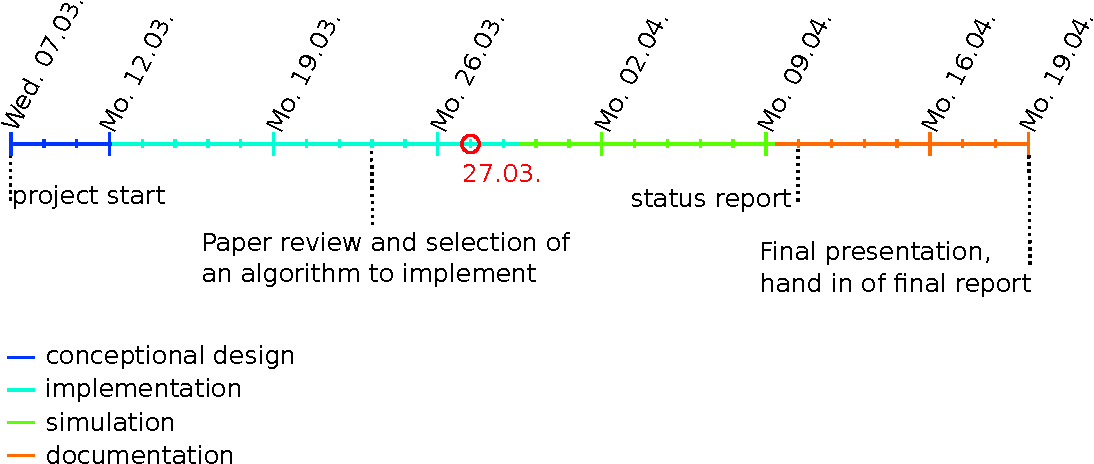
\includegraphics[width=\linewidth]{timeline.pdf}
 \caption{Project timeline}
 \label{fig:project_timeline}
\end{figure}

\begin{table}[h]
\centering
\caption{Project processes}
\label{tab:project_processes}
\begin{tabular}{llllll}
\rowcolor[HTML]{EFEFEF} 
\cellcolor[HTML]{EFEFEF}                          & \multicolumn{2}{c}{\cellcolor[HTML]{EFEFEF}Effort} & \cellcolor[HTML]{EFEFEF}                             & \cellcolor[HTML]{EFEFEF}             &      \\
\rowcolor[HTML]{EFEFEF} 
\multirow{-2}{*}{\cellcolor[HTML]{EFEFEF}Process} & Days                  & Percent                   & \multirow{-2}{*}{\cellcolor[HTML]{EFEFEF}start date} & \multirow{-2}{*}{\cellcolor[HTML]{EFEFEF}due date} & \multirow{-2}{*}{\cellcolor[HTML]{EFEFEF}progress} \\
conceptional design                               & 3.1 d   & 10 \%  & 07.03. & 12.03. & 100 \% \\
implementation                                    & 12.4 d  & 40 \%  & 12.03. & 28.03. & 50 \% \\
\hspace{0.5cm}research                            & 4.65 d  & 15 \%  & 12.03. & 16.03. & 90 \% \\
\hspace{0.5cm}concept                             & 1.55 d  & 5 \%   & 16.03. & 20.03. & 50 \% \\
\hspace{0.5cm}coding                              & 6.2 d   & 20 \%  & 20.03. & 28.03. & 10 \% \\
simulation                                        & 7.75 d  & 25 \%  & 28.03. & 09.04. & 17 \% \\
\hspace{0.5cm}research                            & 4.65 d  & 15 \%  & 28.03. & 30.03. & 50 \% \\
\hspace{0.5cm}setup                               & 1.55 d  & 5 \%   & 30.03. & 02.04. & 0 \% \\
\hspace{0.5cm}simulate setup                      & 1.55 d  & 5 \%   & 02.04. & 09.04. & 0 \% \\
documentation                                     & 7.75 d  & 25 \%  & 09.04. & 17.04. & 0 \% \\
\hspace{0.5cm}analyze results                     & 1.55 d  & 5 \%   & 09.04. & 10.04. & 0 \% \\
\hspace{0.5cm}prepare presentation                & 3.1 d   & 10 \%  & 10.04. & 16.04. & 0 \% \\
\hspace{0.5cm}prepare report                      & 3.1 d   & 10 \%  & 16.04. & 17.04. & 0 \% \\
\end{tabular}
\end{table}

\subsection{Progress}

\begin{figure}[h!]
 \centering
 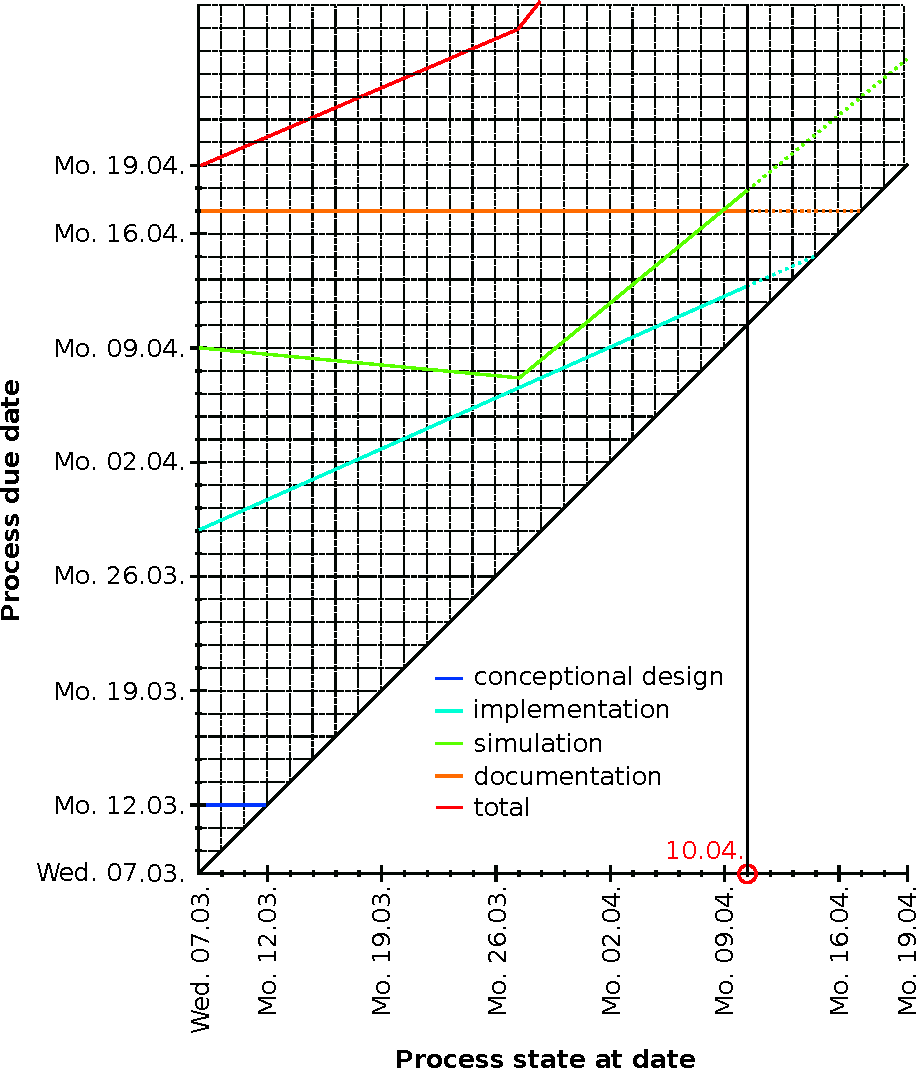
\includegraphics[width=\linewidth]{progress.pdf}
 \caption{Project progress}
 \label{fig:project_progress}
\end{figure}

The progress of the main project processes in table \ref{tab:project_processes} is illustrated in figure \ref{fig:project_progress}. 
The dashed colored lines show a simple estimated future progress of the processes. If the current trend holds on, the project will be
finished approximately 12 working days after the final due date.


\newpage

\section{Presentation of intermediate results}
\subsection{Considered DFBA approaches}\label{ssec:considered_dfba_approaches}

As already discussed in the grant application, we can define the following basic requirements to the implementation of the simulator:
\begin{enumerate}
 \item simulation of co-cultures
 \item in a batch process
 \item with following bacteria cultures: Saccharomyces cerevisiae, Lactobacillus plantarum
 \item starting conditions are parameterized
 \item simulation results include: metabolite densities and biomass of bacteria cultures after a defined time interval
\end{enumerate}
Additional secondary goals are:
\begin{itemize}
 \item generic or automated integration of bacteria models
 \item optimized or even graphical user interface
 \item enhanced model of the fermentation process for more accurate results
\end{itemize}

\vspace{0.5cm}

Zomorri et al. summarizes in \cite{zomorrodi_synthetic_2016} models to predict the behavior of bacteria cultures and introduces
different categories. Three of them are especially
interesting to be used in this project: \textit{steady-state models}, \textit{spatio-temporal models} and \textit{dynamic models}.
\textit{Steady-state models} like compartmentalized community-level metabolic modeling can not be used
since a common objective can not be generally assumed, as it would be in a purely competitive co-cultures
\textit{Spatio-temporal models} have a very high computational effort as they take spacial and temporal varying bacteria densities
into account. As the spacial aspect is not necessarily required in this project a more optimal approach shall be preferred.
The remaining category of \textit{dynamic models} is a well established method to simulate microbial co-cultures in batch processes
and summarizes different extensions to dynamic flux balance analyses methods (DFBA)\cite{zomorrodi_synthetic_2016}. They use genome-
scale models (GEM) to simulate the behavior of the bacteria cultures and add differential equations to model the external system dynamics.

Mehadevan et al. introduces two basic categories of DFBA approaches: \textit{dynamic optimization approach} (DOA) and \textit{static
optimization approach} (SOA)\cite{mahadevan_dynamic_2002}. In DOA a the linear programming problem (LP) which predicts the bacteria
behavior is reformulized to a non-linear programming problem (NLP). This approach has a very high computational effort
\cite{hoffner_reliable_2013} compared to SOA and has only been used for relatively small GEMs with up to 13 modeled fluxes and 8 metabolites
\cite{luo_dynamic_2006} \cite{luo_photosynthetic_2009}.

Mehadevan et al. introduces SOA in \cite{mahadevan_dynamic_2002} as follows: The simulation interval is divided into several intervals and the LP is solved for each
of these time intervals dependent on the metabolite densities. The solution of the LP defines the bacteria growth and metabolite
production at a certain point of time in the simulation time interval. These values are then used to solve the differential equations
which models the external system dynamics. To solve the LP for the next time interval the new calculated, changed metabolite densities
are used. This procedure is repeated until the end of the simulation time interval is reached. This approach makes use of the
assumption that the cell internal dynamics are much faster than the external dynamics. In SOA the behavior of the bacteria is assumed
to be constant during one time interval what leads to a linear approximation approach when solving the system of ordinary differential
equations (ODE), similar to Euler-Cauchy methods.

Höffner et al. adds in \cite{hoffner_reliable_2013} a further group, the \textit{direct approach} (DA) which basically describes methods
similar to SOA which uses an ODE solver instead of the Euler-Cauchy method. Due to the used ODE solver different numerical approximation
methods can be used, not only the linear approximation. A good documented example for this group is the \textit{Dynamic Multispecies
Metabolic Modeling} framework by Zhuang et al. \cite{zhuang_design_2012}.

Henson et al. mentions a third group, \textit{reformulation to a differential-glgebraic equation system} \cite{henson_dynamic_2014}.
It shows also many similarities to SOA with the difference that the LP is reformulized but still solved as a LP embedded within 
the external ODE. The reformulated equation system makes it possible to enhance the efficiency of algorithm compared to SOA and DA
\cite{hoffner_reliable_2013}.

\subsection{DMMM}

\begin{equation}
 \frac{\mathrm d X_j}{\mathrm d t} = \mu_j \alpha_j X_j
\end{equation}
\begin{equation}
 \left[ X \right] = \frac{g}{l}
\end{equation}
\begin{equation}
 \left[ \alpha \right] = \frac{g}{mmol}
\end{equation}
\begin{equation}
 \left[ \mu \right] = \frac{mmol}{g_{DW} h}
\end{equation}

\begin{equation}
 \frac{\mathrm d S_i}{\mathrm d t} = \displaystyle\sum_{j=1}^{N} v_{i,j} X_j
\end{equation}
\begin{equation}
 \left[ v \right] = \frac{mmol}{g_{DW} h}
\end{equation}
\begin{equation}
 \left[ S \right] = \frac{mmol}{l}
\end{equation}

\begin{equation}
 v_{max,i,j} = \frac{V_{max,i,j} S_i}{S_i + K_{i,j}}
\end{equation}
\begin{equation}
 \left[ V \right] = \frac{mmol}{g_{DW} h}
\end{equation}
\begin{equation}
 \left[ K \right] = \frac{mmol}{l}
\end{equation}

To-Do:
\begin{itemize}
 \item mortabilität einbauen: Welches modell nehme ich dafür? Absterben falls growth geht gegen 0? Oder eine Mortabilität als faktor?
 \item Vergleiche $V_{max}$ und K mit geweiligen Paper und checke ob die Gleichungen stimmen
 \item Schreibe bisschen was zu den Michaelis-Menten kinetics
 \item Male ein Bild das die Simulation darstellt (evtl. ähnlich wie im DMMM paper?)
 \item giesse die Optimierung in eine mathematische Beschreibung
 \item erstelle Pseudocode um den Algorithmus zu beschreiben
\end{itemize}






\subsection{Approach selection}

\begin{table}[]
\centering
\caption{Rating of considered DFBA methods}
\label{tab:rating_of_DFBA_methods}
\begin{tabular}{llll}
\rowcolor[HTML]{EFEFEF} 
Method                                                                                                 & \begin{tabular}[c]{@{}l@{}}comp.\\ effort\end{tabular} & \begin{tabular}[c]{@{}l@{}}impl.\\ complexity\end{tabular} & flexibility \\
dynamic optimization approach (DOA)                                                                    & high                                                   & medium-high                                                & ?           \\
static optimization approach (SOA)                                                                     & low                                                    & low                                                        & low         \\
direct approach (DA)                                                                                   & medium                                                 & low                                                        & medium      \\
\begin{tabular}[c]{@{}l@{}}reformulation to a differential-glgebraic\\ equation system\end{tabular} & low-medium                                             & high                                                       & ?          
\end{tabular}
\end{table}

The described DFBA methods in section \ref{ssec:considered_dfba_approaches} were rated based on the given information in the above mentioned
papers, see table \ref{tab:rating_of_DFBA_methods}.

DOA can not be used due to its high computational effort and medium-high implementation complexity. The approach which uses
\textit{reformulation to a differential-glgebraic equation system} is currently available in matlab code and must be implemented
in python in this project. Due to the high implementation complexity this approach will also be excluded.
The remaining methods, SOA and DA, have similar ratings but as DA is more flexible as different ODE solvers can be used this approach
seems more sustainable. Besides its flexibility the DA implementation DMMM by Zhuang et al. \cite{zhuang_design_2012} can be publicly
accessed and they provide a good documentation which will facilitate the implementation in this project.

\section{Outlook}

Due to unexpected high effort in the research of simulation algorithms and technical problems the project progress is not as fast
as expected (see figure \ref{fig:project_progress}). It is assumed that the technical problems were a single event and will not
occure again, so this will not lead to further delay. As the high effort part in research for simulation algorithms is done, it
can also be assumed that this will not cause further delay, too. Under these assumptions (no further delay in all processes) the
project delay can be reduced from 12 to 6 days.

To catch up the remaining delay, a higher focus was set to choose a simulation algorithm with less implementation complexity.
Furthermore, if this is not enough to catch up the delay, the complexity of the later simulations can be further reduced.

\vspace{0.5cm}
The subsequent steps include:
\begin{itemize}
 \item research on modeling uptake limits dependent on metabolite densities in the substrate using Michaelis–Menten kinetics
 \item mathematical formulation of the model
 \item implementation of the simulation algorithm
\end{itemize}




\newpage

\printbibliography

\end{document}
